
\def \Subject {گزارش جمع آوری داده }
\def \Course {درس یادگیری ماشین}
\def \Author {کسرا سینایی، امیرحسین افخمی، پارسا شفیعی و }
\def \Report {گزارش فاز اول}
\def \StudentNumber {۸۱۰۶۹۶۲۵۴، ، و }

\begin{center}
\vspace{.4cm}
{\bf {\huge \Subject}}\\
{\bf \Large \Course}
\vspace{.2cm}
\end{center}
{\bf \Author }  \\
{\bf شماره دانشجویی:\ \StudentNumber}
\hspace{\fill} 
{\Large \Report} \\
\hrule
\vspace{0.8cm}

\clearpage

%\huge{\Subject}\\[1.5 cm]
%\chapterauthor{\Author~ : \StudentNumber}
\par
 خواهش‌مند است نام و نام خانوادگی ، سری تمرینات، شماره داشجویی خود در ابتدای این فایل را با دقت پر کنید.

\section{سوال 1}
\subsection{کد سوالات}

 برای نمایش کد موجود در فایل پاسخ خود،
 فایل را در پوشه 
 \texttt{sources}
 آپلود کرده و به صورت زیر آن را نمایش دهید. 
 
\begin{latin}
\begin{listing}[ht]
    \inputminted{octave}{sources/partition.py}
    \caption{External file code}
    \label{listing:}
\end{listing}
\end{latin}

\subsection{فرمول ها}
\par
برای نمایش فرمول ریاضی می‌توانید از نمونه زیر استفاده کنید:
		\begin{equation}
		|\delta V |=\left[ \frac{E}{4}\right] \ \frac{\delta R}{R}, \ \ where\ E=10\ V, k=2.5
		\end{equation}
\clearpage


\subsection{جدول}
\par
برای ساختن جدول 
 می‌توانید از مثال زیر در گزارش خود
  \ref{t1}
   استفاده کنید :


\begin{table}[!h]
\centering
\begin{latin}
\begin{tabular}{|c|c|c|c|}
	\hline
	$\delta R $ & $\delta R/R \ (10^{-3})$ \  & $ \delta V $(mV) & Theoretical $\delta$ V (mV) \\
	\hline\hline
	0 & 0.00 & 0.05 & 0.00\\
	\hline
	1 & 8.33 & 20.00 &20.83\\
	\hline
	2 & 16.67 & 40.90 &41.67\\
	\hline
	3 & 25.00 & 61.40 &62.50\\
	\hline
	4 & 33.33 & 81.90 &83.33\\
	\hline
	5 & 41.67 & 102.00 &104.17\\
	\hline
	6 & 50.00 & 122.30 &125.00\\
	\hline
	7 & 58.33 & 142.00 &145.83\\
	\hline
	8 & 66.67 & 161.70 &166.67\\
	\hline
	9 & 75.00 & 181.50 &187.50\\
	\hline
\end{tabular}
\end{latin}
\caption{نتایج اندازه گیری های آزمایش 1}
\label{t1}
\end{table}

\subsection{شکل}
\par
همچنین برای اضافه کردن شکل می‌توانید از شکل زیر استفاده کنید و برای ارجاع دادن به بصورت شکل
 \ref{fig:dynamicprogramming}
 استفاده کنید.
 همچنین برای درج کلمات انگلیسی در پاراگراف فارسی می‌توان به این شکل
 \lr{English Text}
 یا برای تاکید به این شکل
 \grayBox{English Text}
 عمل کرد.
\begin{figure}[h!]
    \centering
    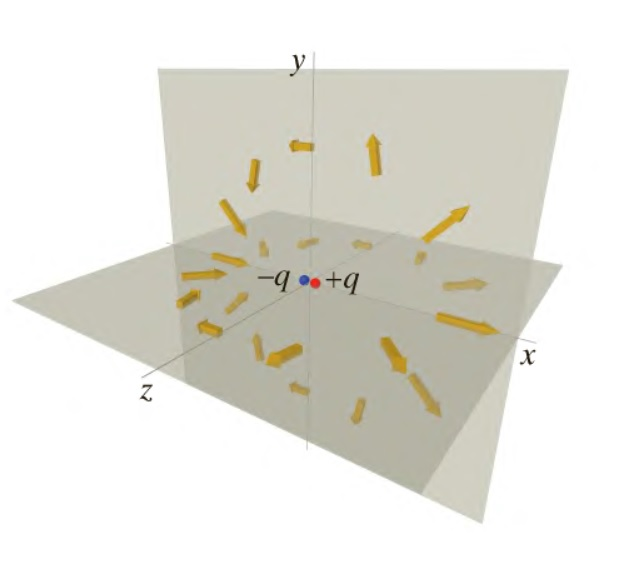
\includegraphics[width=0.5\linewidth]{images/dipole.jpg}
    \caption{دوقطبی الکتریکی}
    \label{fig:dynamicprogramming}
\end{figure}\\




